Quadcopter control is a complex, yet interesting problem. One of the reasons why this control problem is challenging is the fact that a quadcopter has six degrees of freedom, but only four inputs which affects the linearity of the dynamics and makes the quadcopter underactuated. One other important thing to mention is that quadcopters, unlike ground vehicles, have very little friction that prevents their motion, so they have to provide their own damping in order to be able to stop or maintain stability.

This chapter will give a general overview on the pieces of technical equipment which we are using and show what the purpose of each one is. It will also present how our scopes - hovering and maneuvering - can be achieved by designing and implementing a control system. A solution in terms of the structure of our control system will be identified. We will also delve into the basic working principle of a quadcopter/flight dynamics.

\section{Physical Setup}
\subsection{Motors} \label{Motors}
Controlling a quadcopter can be done efficiently by using high-quality motors with fast response, which will ensure more of a stable flight. The motors must also be powerful enough to be able to lift the quadcopter and perform the required aerial movements. 

The motor that we are using is the Turnigy Multistar Brushless Motor seen in Figure \ref{motor}.

\begin{figure}[H]
  \centering
    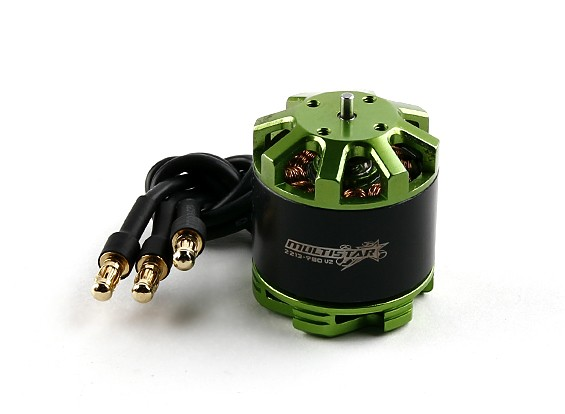
\includegraphics[width=0.5\textwidth]{images/motor.jpg}
	\caption{Turnigy Multistar 2213-980 V2 Brushless Motor}
	\label{motor}
\end{figure}

\subsection{Propellers}
The propellers don't have such strict requirements as the motors. They are needed to be light and have a size and lift potential in order for the quadcopter to hover at less than 50\% of the motor capacity. For our quadcopter, we are using plasting 10x4.5'' propellers with light weight - 60g. They have a length of 254 mm and a pitch inclination of 114mm. They can be seen in Figure \ref{propeller}.

\begin{figure}[H]
  \centering
    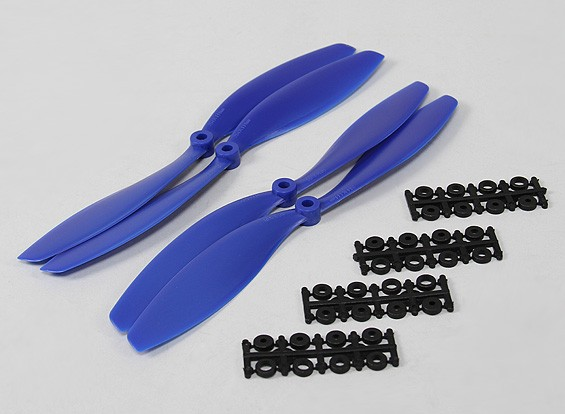
\includegraphics[width=0.5\textwidth]{images/propeller.jpg}
	\caption{Hobbyking Slowfly Propeller 10x4.5}
	\label{propeller}
\end{figure}

\subsection{Electric Speed Controller}
Electronic Speed Controller (ESC) is a widely used device in rotorcrafts. The purpose of an ESC is to vary the electric motor's speed. They also come with programmable features, such as braking or selecting appropriate type of battery. We need the ESC to have a fast response, for the same reasons mentioned for the motors in Section \ref{Motors}. The ESC that we are using is the TURNIGY Plush 30A which is shown in Figure \ref{esc}.
 
\begin{figure}[H]
  \centering
    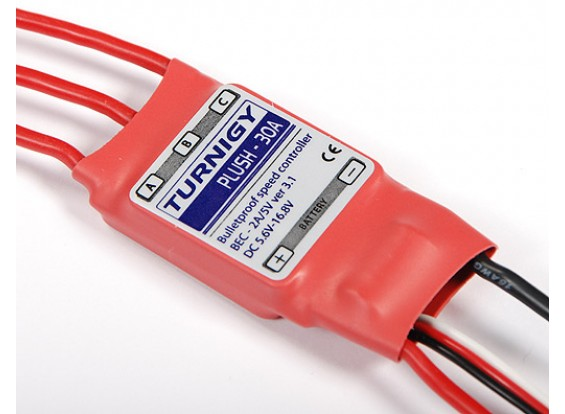
\includegraphics[width=0.5\textwidth]{images/esc.jpg}
	\caption{TURNIGY Plush 30A Speed Controller}
	\label{esc}
\end{figure}

\subsection{APM Flight Controller}
ArduPilotMega (APM) is an open source unmanned aerial vehicle (UAV) platform which is able to control autonomous multicopters. It is illustrated in Figure \ref{ardupilot}. The system was improved uses Inertial Measurement Unit (IMU) - a combination of accelerometers, gyroscopes and magnetometers. The "Ardu" part of the project name shows that the programming can be done using Arduino open-source language.

\begin{figure}[H]
  \centering
    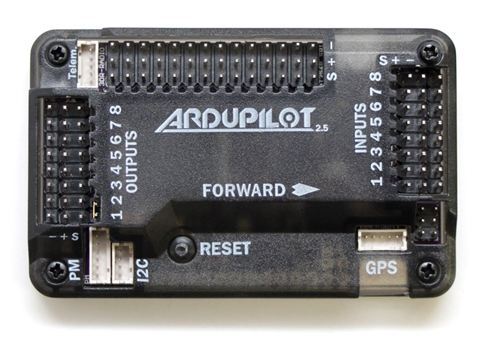
\includegraphics[width=0.5\textwidth]{images/ardupilot.jpg}
	\caption{APM 2.5 board}
	\label{ardupilot}
\end{figure}

\subsection{Power Distribution Board}
To reduce the number of connections straight to the battery, we used the a power distribution board made for a previous project. A board like this is an easy solution since it enables us to connect the four ESCs directly to the board and then connect the board to the battery.

\subsection{Battery}
To power up our quadcopter, we will use a TURNIGY nano-tech Lipoly battery, which can be seen in Figure \ref{battery}. Higher voltage under load, straighter discharge curves and excellent performance are the factors that make it suitable for our project. 

\begin{figure}[H]
  \centering
    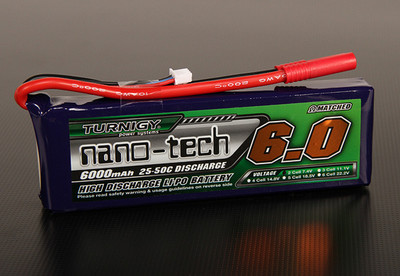
\includegraphics[width=0.5\textwidth]{images/battery.jpg}
	\caption{Turnigy nano-tech 6000mah 3S 25~50C Lipo Pack}
	\label{battery}
\end{figure}

\clearpage

\section{Flight Dynamics}

In order to put a working quadcopter together, it is important to understand the basic flight dynamics - the forces affecting the vehicle as well as the motors' speed effect.
There are 4 main forces affecting quadcopter - or any airborne vehicle, for that matter - thrust, lift, draw and drop. See figure \ref{droneForces}.
\begin{figure}[H]
  \centering
    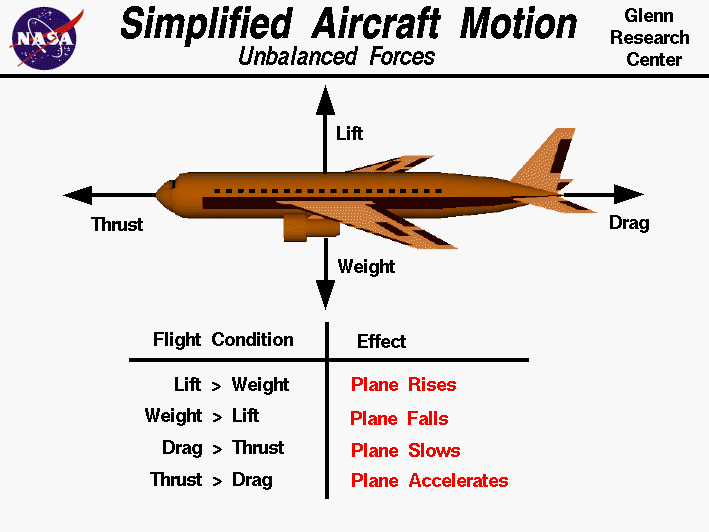
\includegraphics[width=0.7\textwidth]{images/droneForces.png}
	\caption{Forces affecting an airborne vehicle\cite{dForces}}
	\label{droneForces}
\end{figure}

The drop - or the gravitational force - affects the vehicle at all times. As any object on Earth, its mass is driven towards the centre of the planet. This force, \textit{$F_g$}, is always equal to: $F_g = mg$, where \textit{m} is the mass of the drone and \textit{g} is the gravitational constant.

The thrust is the force generated by the motors that is allowing the vehicle to move towards its heading. In case of a quadcopter, this force only exists when the force generated by the motors is uneven.

The lift force, following Bernoulli's principle, is created through a difference in the air pressure above and below the motor. Quadcopter's motors constantly generate lift force, which must be higher than the drop force in order for the vehicle to take flight.

Draw force is the resistance created by the air as the vehicle moves through it. It opposes the thrust force and therefore must be lower than the thrust force in order for the quadcopter to move on. In cases when is no wind, such as indoors area, this force can be disregarded due to lack of wind.

A powered off motors is only affected by the drop force and therefore stays on the ground. In order to lift it up, we need to understand the relationship between quadcopter and the thrust to weight ratio - or TWR for short. This ratio can be determined by equation $F_t/F_g$ and describes the vehicle's ability to move up. With TWR expressed as a number, assuming that each motor generates equal amount of thrust, three cases can be identified:
\begin{enumerate}
\item TWR < 1: The gravitational force is higher than the lift force and therefore the quadcopter is drawn towards the ground.
\item TWR = 1: The forces are equal, causing quadcopter's altitude to stay constant.
\item TWR > 1: The thrust is higher than drop force, allowing vehicle to move upwards.
\end{enumerate}

Therefore, in order to get a quadcopter up in the air, it is necessary to generate enough thrust for TWR ration to be higher than one. In order to land it, the TWR must be smaller than 1, allowing the quadcopter to move downwards.

Moving on, it is necessary to understand the effects that motor speeds have on the vehicle. While equal amount of force generated by every motor will result in a movement on vertical axis, differences in motor speeds will create a change in quadcopter's pitch, roll or yaw. These three motions can be seen in figure \ref{droneMotions}.
\begin{figure}[H]
  \centering
    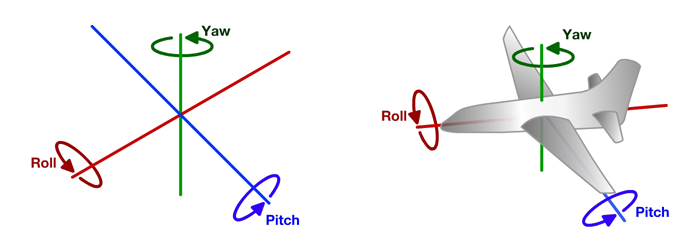
\includegraphics[width=0.7\textwidth]{images/droneMotions.png}
	\caption{Pitch, roll and yaw motions in a 3-dimensional plane\cite{dMotions}}
	\label{droneMotions}
\end{figure}

To examine the consequences of different motor speeds, let's assume there's a simple quadcopter with all 4 motors placed at equal distances from the centre. An example can be seen in figure \ref{droneIdle}.
\begin{figure}[H]
  \centering
    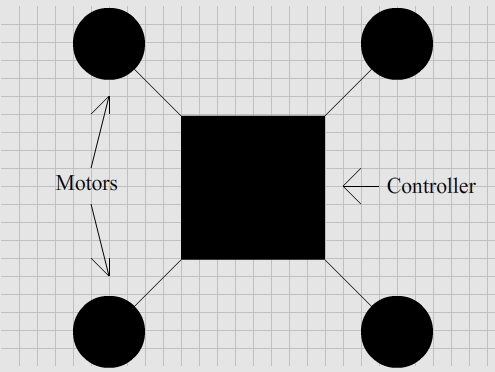
\includegraphics[width=0.7\textwidth]{images/droneIdle.png}
	\caption{A quadcopter viewed from top}
	\label{droneIdle}
\end{figure}

The direction of rotation and produced torque as well as the amount of force generated by the motors affect the quadcopter's movement. See figure \ref{droneDirections} for an example in an idle - or hovering - position.
\begin{figure}[H]
  \centering
    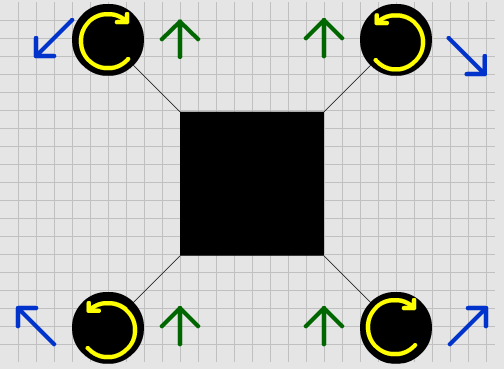
\includegraphics[width=0.7\textwidth]{images/droneDirections.png}
	\caption{Motor direction overview}
	\label{droneDirections}
\end{figure}
Here, the yellow arrows indicate the direction of rotation, the blue arrows show the direction of torque and the green arrows display the amount of force generated by the motors.

By controlling the speed at which the motors rotate, it is possible to change how quadcopter moves. Movement can be broken down in 3 separate sets of motor speeds:

1) If the two back motors rotate faster than the two frontal motors, the quadcopter will pitch forward. Switching the speeds will result in aft pitch. The required change in speeds for a pitch forward can be seen in figure \ref{dronePitch}.
\begin{figure}[H]
  \centering
    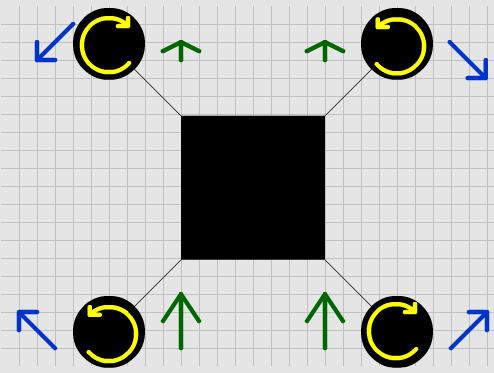
\includegraphics[width=0.7\textwidth]{images/dronePitch.png}
	\caption{Motor RPM requirements for a pitch forward}
	\label{dronePitch}
\end{figure}
2) If the two left motors have higher RPM than the two motors on the right side, the vehicle will roll to the right. Swapping the speeds differences will result in a roll to the left. See figure \ref{droneRoll} for an example of a roll to the right.
\begin{figure}[H]
  \centering
    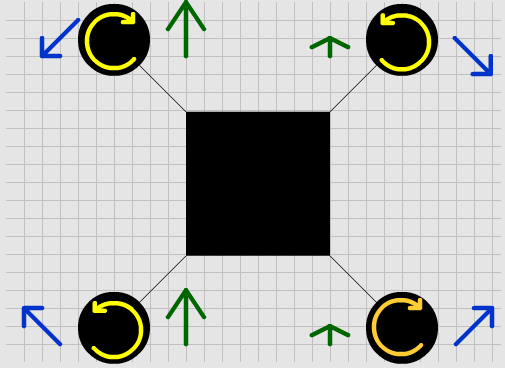
\includegraphics[width=0.7\textwidth]{images/droneRoll.png}
	\caption{RPM requirements for a roll to the right}
	\label{droneRoll}
\end{figure}
3) Increasing the speed of one of the diagonal pair of the motors will result in yaw to the direction of the torque of the motors. The copter will then spin around its axis. Motor speed changes causing a yaw to the right can be seen in figure \ref{droneYaw}.
\begin{figure}[H]
  \centering
    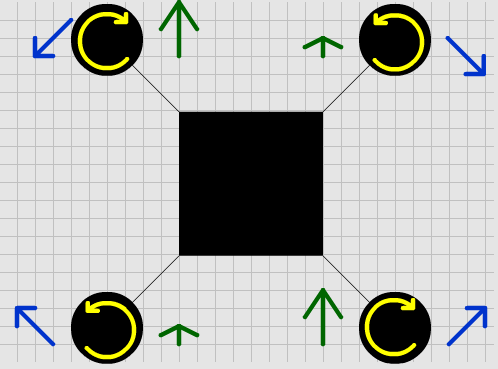
\includegraphics[width=0.7\textwidth]{images/droneYaw.png}
	\caption{The two diagonal motors with increased RPM cause yaw to the right}
	\label{droneYaw}
\end{figure}
